\documentclass[conference]{IEEEtran}
\IEEEoverridecommandlockouts

\usepackage{cite}
\usepackage{amsmath,amssymb,amsfonts}
\usepackage{algorithmic}
\usepackage{graphicx}
\usepackage{textcomp}
\usepackage{xcolor}
\usepackage{booktabs}
\usepackage{array}
\usepackage{url}
\usepackage{hyperref}
\usepackage{listings}
\usepackage{tikz}
\usepackage{pgfplots}
\pgfplotsset{compat=1.18}
\usepackage{multirow}
\usepackage{balance}

\lstset{
  basicstyle=\ttfamily\footnotesize,
  breaklines=true,
  frame=single,
  backgroundcolor=\color{gray!10},
  keywordstyle=\color{blue},
  commentstyle=\color{green!60!black},
  stringstyle=\color{orange}
}

\def\BibTeX{{\rm B\kern-.05em{\sc i\kern-.025em b}\kern-.08em
    T\kern-.1667em\lower.7ex\hbox{E}\kern-.125emX}}

\begin{document}

\title{LaunchMind: An Autonomous Multi-Agent System for\\
End-to-End AI-Driven Startup Launch Automation}

\author{
\IEEEauthorblockN{Bilal Aleem}
\IEEEauthorblockA{\textit{Department of Computer Science} \\
\textit{FAST-NUCES} \\
Islamabad, Pakistan \\
bilalaleem5@github.com}
}

\maketitle

\begin{abstract}
The process of launching a technology startup demands simultaneous expertise across product design, software engineering, marketing, and quality assurance—a combination rarely possessed by a single individual or small team. This paper presents \textbf{LaunchMind}, an autonomous Multi-Agent System (MAS) that orchestrates a team of specialized AI agents to automate the complete startup launch pipeline from ideation to deployment artifacts. The system comprises five cooperating agents—CEO, Product, Engineer, Marketing, and QA—communicating via a persistent SQLite-backed message bus and a shared memory scratchpad. Each agent is powered by a large language model (LLM) and equipped with domain-specific tools: the Engineer Agent integrates with the GitHub API to create branches and pull requests autonomously, while the Marketing Agent delivers real-time launch notifications via the Slack API. A dedicated QA Ethics Guardrail agent evaluates all generated content for factual accuracy, professional tone, and absence of deceptive claims, scoring outputs on a 0--10 ethics scale before the CEO Agent approves final delivery. Empirical evaluation across five distinct startup scenarios demonstrates a \textbf{100\% task-completion rate} with an average end-to-end latency of \textbf{11--13 seconds} and a mean ethics score of \textbf{9.0/10}. The system is implemented in Python with a companion high-performance Rust module for message bus operations, and all artifacts—including GitHub pull requests and Slack notifications—are verifiably produced by the agents without human intervention. LaunchMind demonstrates that structured multi-agent orchestration with built-in ethical guardrails can dramatically reduce the time and expertise required to launch an AI-powered product.
\end{abstract}

\begin{IEEEkeywords}
Multi-Agent Systems, Autonomous AI, LLM Orchestration, Startup Automation, Ethical AI, GitHub API, Slack Integration, CEO Agent, QA Guardrails, Agentic Workflows
\end{IEEEkeywords}

%% ─────────────────────────────────────────────────────────
\section{Introduction}
\label{sec:intro}
%% ─────────────────────────────────────────────────────────

Launching a technology startup in the modern era involves a coordinated sequence of activities spanning market research, product specification, software development, marketing copywriting, and rigorous quality assurance. Each of these activities traditionally requires a domain expert, making early-stage startups dependent on either co-founder teams with complementary skills or expensive outsourcing. The rise of large language models (LLMs) has opened the possibility of delegating cognitive work across multiple artificial agents, each specializing in one domain of this pipeline.

Existing single-agent systems—such as AutoGPT \cite{autogpt2023} and BabyAGI \cite{babyagi2023}—have demonstrated that LLMs can autonomously decompose and execute complex tasks. However, these systems suffer from context window limitations when tasks grow complex, lack role specialization, and often produce unchecked outputs that may be factually misleading or ethically problematic. Frameworks such as LangChain \cite{langchain2022} and CrewAI \cite{crewai2024} provide agent orchestration primitives but do not offer domain-specific tooling, persistent shared memory with audit trails, or integrated ethical evaluation.

This paper presents \textbf{LaunchMind}, a purpose-built MAS that directly addresses these gaps for the startup-launch domain. The system makes the following specific contributions:

\begin{itemize}
    \item \textbf{Role-specialized agent hierarchy:} A CEO orchestrator delegates tasks to four specialist agents (Product, Engineer, Marketing, QA), each with dedicated prompts, tools, and output schemas.
    \item \textbf{Persistent SQLite message bus:} All inter-agent messages are persisted in a relational database, providing a complete, queryable audit log suitable for debugging and compliance.
    \item \textbf{Shared memory scratchpad:} Agents read and write to a shared key-value memory store, enabling context propagation across agent boundaries without bloating individual context windows.
    \item \textbf{Real-world API integrations:} The Engineer Agent autonomously creates GitHub branches, commits code, and opens pull requests. The Marketing Agent posts formatted launch announcements to Slack channels.
    \item \textbf{Built-in ethics guardrail:} The QA Agent evaluates every content artifact against a professional-tone rubric, assigns a numeric ethics score, and blocks delivery if the score falls below threshold.
    \item \textbf{Empirical validation:} We evaluate the system across five diverse startup scenarios, reporting latency, ethics scores, and task-completion rates.
\end{itemize}

The remainder of the paper is organized as follows. Section~\ref{sec:related} reviews related work. Section~\ref{sec:arch} describes the system architecture. Section~\ref{sec:impl} discusses implementation details. Section~\ref{sec:eval} presents experimental results. Section~\ref{sec:ethics} discusses ethical considerations. Section~\ref{sec:future} outlines future directions, and Section~\ref{sec:conclusion} concludes.

%% ─────────────────────────────────────────────────────────
\section{Related Work}
\label{sec:related}
%% ─────────────────────────────────────────────────────────

\subsection{Single-Agent LLM Systems}

AutoGPT \cite{autogpt2023} pioneered autonomous LLM task execution by giving a single agent a goal and letting it self-prompt through tool calls. While powerful, it struggles with long-horizon tasks requiring specialized knowledge because a single agent must maintain all context. BabyAGI \cite{babyagi2023} improved on this with a task-queue architecture but similarly lacks inter-agent specialization.

\subsection{Multi-Agent Frameworks}

MetaGPT \cite{metagpt2023} introduced role-based agents for software engineering workflows, assigning agents to roles such as Product Manager, Architect, and Engineer. Our work extends this concept to the startup-launch domain and adds persistent message logging and external API integrations not present in MetaGPT. AgentVerse \cite{agentverse2023} demonstrates multi-agent collaboration for problem-solving but does not address real-world tool integration or ethical evaluation. CAMEL \cite{camel2023} explores role-playing for agent communication but uses simulated dialogues rather than structured JSON message protocols with database persistence.

\subsection{LLM Orchestration Frameworks}

LangChain \cite{langchain2022} provides composable agent abstractions and tool connectors, and LangGraph extends it with stateful graph-based workflows. CrewAI \cite{crewai2024} offers a higher-level crew abstraction where agents collaborate via a shared context. LaunchMind differs from these frameworks in that it is domain-specific, includes a CEO decision-making layer with approval loops, and embeds a dedicated ethics evaluation step prior to every external API action.

\subsection{Ethical AI and Safety Guardrails}

Constitutional AI \cite{bai2022constitutional} trains LLMs with self-critique loops to reduce harmful outputs. Our QA Ethics Agent operationalizes a similar philosophy at the system level: rather than relying solely on model alignment, it adds an independent agent that scores and gates output delivery, providing an auditable safety layer.

%% ─────────────────────────────────────────────────────────
\section{System Architecture}
\label{sec:arch}
%% ─────────────────────────────────────────────────────────

\subsection{Overview}

LaunchMind adopts a hierarchical MAS architecture as illustrated in Fig.~\ref{fig:arch}. The CEO Agent acts as the central orchestrator, receiving the initial startup idea and decomposing it into sub-tasks dispatched to specialist agents. All agents communicate exclusively through the Message Bus, and shared contextual data is stored in the Shared Memory layer. Before the CEO Agent approves any external action, the QA Ethics Guardrail agent reviews all generated content.

\begin{figure}[htbp]
\centering
% Architecture diagram described textually since TikZ is used
\begin{tikzpicture}[
  node distance=1.1cm and 1.6cm,
  box/.style={draw, rounded corners, minimum width=2.0cm, minimum height=0.7cm,
               font=\small, align=center, fill=teal!15},
  ext/.style={draw, rounded corners, minimum width=2.0cm, minimum height=0.7cm,
               font=\small, align=center, fill=blue!10},
  arr/.style={->, thick}
]
  % Nodes
  \node[box] (ceo)  {CEO Agent};
  \node[box, above left=of ceo]  (product)  {Product\\Agent};
  \node[ext, above right=of ceo] (engineer) {Engineer\\Agent\\(GitHub)};
  \node[ext, below right=of ceo] (marketing){Marketing\\Agent\\(Slack)};
  \node[box, below=1.4cm of ceo] (qa)       {QA Ethics\\Guardrail};
  \node[box, above=1.4cm of ceo] (msgbus)   {Message Bus\\(SQLite)};
  \node[box, left=1.6cm of qa]   (memory)   {Shared\\Memory};
  \node[box, below=1.0cm of qa]  (launch)   {Launch\\Success};

  % Arrows
  \draw[arr] (ceo)    -- (msgbus);
  \draw[arr] (msgbus) -- (ceo);
  \draw[arr] (ceo)    -- (product);
  \draw[arr] (product)-- (ceo);
  \draw[arr] (ceo)    -- (engineer);
  \draw[arr] (engineer)--(ceo);
  \draw[arr] (ceo)    -- (marketing);
  \draw[arr] (marketing)--(ceo);
  \draw[arr] (ceo)    -- (qa);
  \draw[arr] (qa)     -- (ceo);
  \draw[arr] (qa)     -- (memory);
  \draw[arr] (memory) -- (qa);
  \draw[arr] (qa)     -- (launch);
\end{tikzpicture}
\caption{LaunchMind Multi-Agent System Architecture. The CEO Agent orchestrates all specialist agents via a persistent SQLite Message Bus. Shared Memory enables cross-agent context propagation. The QA Ethics Guardrail gates all outputs before final delivery.}
\label{fig:arch}
\end{figure}

\subsection{Agent Roles and Responsibilities}

\subsubsection{CEO Agent}
The CEO Agent is the entry point and decision authority. It receives the startup idea as a natural-language string, formulates a launch strategy, and issues structured TASK messages to each specialist. Upon receiving RESULT messages, the CEO evaluates whether the task cycle is complete or requires revision. After QA approval, the CEO Agent writes a summary report and terminates the run.

\subsubsection{Product Agent}
The Product Agent generates a structured product specification containing: value proposition, key features (typically 3--5 items), target user personas, and a competitive differentiation statement. Its output is a validated JSON object conforming to a predefined schema, ensuring downstream agents can parse and utilize the spec reliably.

\subsubsection{Engineer Agent}
The Engineer Agent consumes the product specification and generates a landing-page HTML artifact. It then invokes the GitHub REST API to: (1) create a new feature branch named \texttt{agent-landing-page-<hash>}, (2) commit the generated HTML file, and (3) open a pull request titled \texttt{Automated PR: Initial Landing Page} with a description attributing authorship to the agent. The PR URL is returned as the agent's RESULT payload and propagated to all downstream agents via Shared Memory.

\subsubsection{Marketing Agent}
The Marketing Agent produces marketing copy including a product tagline, a one-paragraph description, and a launch announcement. It then invokes the Slack Web API to post a formatted message to a designated \texttt{\#launches} channel. The Slack message embeds the GitHub PR link, the QA verdict, and the product tagline, providing the team with a single-pane-of-glass launch notification.

\subsubsection{QA Ethics Guardrail Agent}
The QA Agent is the system's safety layer. It receives all generated content artifacts—HTML, marketing copy, and product spec—and evaluates them against four criteria: (a) professional tone, (b) absence of deceptive or exaggerated claims, (c) clarity and readability, and (d) alignment with the original idea. Each criterion is scored 0--10 and the scores are averaged. If the aggregate ethics score falls below 7.0, the agent returns a FAIL verdict along with specific issues, prompting the CEO to request revisions. A PASS verdict (score $\geq$ 7.0) allows the CEO to finalize the run. In all evaluated scenarios, the system achieved a score of 9/10 with the justification: \textit{"Professional tone, no deceptive claims, and clear language used."} The QA Agent also posts an inline review comment on the GitHub PR summarizing its findings.

\subsection{Communication Protocol}

All inter-agent communication is mediated by the Message Bus, implemented as an SQLite database table with the schema shown in Listing~\ref{lst:schema}.

\begin{lstlisting}[language=SQL, caption={Message Bus Database Schema}, label={lst:schema}]
CREATE TABLE messages (
  id        INTEGER PRIMARY KEY AUTOINCREMENT,
  timestamp TEXT    NOT NULL,
  from_agent TEXT   NOT NULL,
  to_agent   TEXT   NOT NULL,
  msg_type   TEXT   NOT NULL,  -- TASK | RESULT | CONFIRMATION
  payload    TEXT   NOT NULL   -- JSON string
);
\end{lstlisting}

Each message carries a \texttt{msg\_type} field with one of three values: \textbf{TASK} (a directive from one agent to another), \textbf{RESULT} (the output of a completed task), or \textbf{CONFIRMATION} (an acknowledgment or approval signal). The payload field contains a JSON-serialized object specific to each message type. This design ensures that the complete agent dialogue is persistently recorded and can be replayed or audited at any point.

\subsection{Shared Memory}

The Shared Memory module is a Python dictionary that is accessible to all agents within a single MAS run. It stores canonical values such as the current startup idea, the product spec, the GitHub PR URL, and the QA verdict. Agents read from Shared Memory to avoid re-requesting already-computed context and write to it when they produce new persistent facts. This prevents context-window bloat: agents only receive the subset of memory relevant to their current task.

%% ─────────────────────────────────────────────────────────
\section{Implementation}
\label{sec:impl}
%% ─────────────────────────────────────────────────────────

\subsection{Technology Stack}

LaunchMind is implemented primarily in \textbf{Python 3.11}, with a companion \textbf{Rust} module that provides high-throughput message serialization and SQLite write operations. The repository language breakdown is: Rust 76.0\%, Python 18.2\%, HTML 5.0\%, and other 0.8\%. The Python codebase handles agent logic and API integrations, while the Rust component provides a safe, performant backend for concurrent message bus writes—important when multiple agents attempt to log results simultaneously.

\subsection{LLM Backend}

Each agent is backed by an LLM API call. The system is designed to be model-agnostic: the agent configuration specifies model endpoint, temperature, and system prompt independently per agent. In the reported experiments, all agents used a GPT-class model via the OpenAI-compatible API with temperature 0.7 for creative agents (Product, Marketing) and 0.2 for precision-critical agents (Engineer, QA).

\subsection{GitHub Integration}

The Engineer Agent uses the \texttt{PyGitHub} library to authenticate with a Personal Access Token (PAT) stored as an environment variable. The agent programmatically: creates a branch from \texttt{main}, encodes the HTML content as base64, commits it via the \texttt{create\_file} API, and opens a PR with an auto-generated description. The PR is marked as \textit{"Ready to merge"} and includes zero merge conflicts, as the branch diverges only with new files. The GitHub Actions workflow (\texttt{.github/} directory in the repository) is configured to run automated checks on agent-created PRs.

\subsection{Slack Integration}

The Marketing Agent uses the Slack Web API (\texttt{chat.postMessage}) with a bot OAuth token. Messages are formatted using Slack's Block Kit to include a header banner, a two-column metadata section (GitHub PR link and QA Status), and an embedded GitHub PR preview card generated by Slack's URL unfurling feature.

\subsection{Orchestration Loop}

The CEO Agent implements a finite-state machine with states: \texttt{PLANNING} $\rightarrow$ \texttt{PRODUCT\_SPEC} $\rightarrow$ \texttt{ENGINEERING} $\rightarrow$ \texttt{MARKETING} $\rightarrow$ \texttt{QA\_REVIEW} $\rightarrow$ \texttt{COMPLETE}. The loop is synchronous within each scenario run. Listing~\ref{lst:ceo_loop} shows a simplified view of the orchestration logic.

\begin{lstlisting}[language=Python, caption={Simplified CEO Orchestration Loop}, label={lst:ceo_loop}]
def run_mas(idea: str):
    memory["idea"] = idea
    spec = product_agent.run(idea)
    memory["spec"] = spec
    
    pr_url = engineer_agent.run(spec)
    memory["pr_url"] = pr_url
    
    marketing = marketing_agent.run(spec)
    memory["marketing"] = marketing
    
    qa_result = qa_agent.run(memory)
    
    if qa_result["verdict"] == "pass":
        slack_agent.notify(memory)
        return {"status": "SUCCESS", **memory}
    else:
        raise QAFailureError(qa_result["issues"])
\end{lstlisting}

\subsection{Error Handling and Retry Logic}

Each agent wraps its LLM call in a try-except block with up to three retries using exponential backoff. If the LLM returns malformed JSON (which fails schema validation), the agent re-prompts with an explicit correction instruction. GitHub and Slack API failures raise exceptions that propagate to the CEO Agent, which logs them to the message bus and terminates the run with a FAILURE status.

%% ─────────────────────────────────────────────────────────
\section{Experimental Evaluation}
\label{sec:eval}
%% ─────────────────────────────────────────────────────────

\subsection{Experimental Setup}

We evaluated LaunchMind across five startup scenarios of varying domains and complexity. Each scenario was run on a Windows 11 machine (Intel Core i7, 16 GB RAM) with network access to the GitHub and Slack APIs. We measured: (1) end-to-end wall-clock latency from idea submission to Slack notification delivery, (2) the QA ethics score assigned by the QA Agent, (3) the number of inter-agent messages logged to the SQLite bus, and (4) whether the run concluded with a PASS verdict (task-completion binary). All five scenarios completed successfully without any manual intervention.

\subsection{Scenarios Tested}

\begin{enumerate}
    \item \textbf{Generic AI Automation} — A general-purpose AI automation platform; used as baseline.
    \item \textbf{ZetaMize Test Idea} — Sales analytics tool targeting SMEs.
    \item \textbf{ZetaMize AI Sales OS} — High-end terminal UI-based sales operating system for enterprise users.
    \item \textbf{Intellibot} — An AI chatbot for customer engagement and business intelligence.
    \item \textbf{Sell Smarter, Not Harder} — A marketing automation platform combining AI-powered cold outreach and analytics.
\end{enumerate}

\subsection{Quantitative Results}

Table~\ref{tab:results} presents the per-scenario results. All five scenarios passed QA evaluation on the first attempt with no revision cycles required, yielding a \textbf{100\% first-pass success rate}.

\begin{table}[htbp]
\centering
\caption{Per-Scenario Experimental Results}
\label{tab:results}
\renewcommand{\arraystretch}{1.2}
\begin{tabular}{>{\raggedright}p{2.1cm} c c c c}
\toprule
\textbf{Scenario} & \textbf{Latency (s)} & \textbf{Ethics} & \textbf{Messages} & \textbf{Verdict} \\
\midrule
AI Automation        & 11 & 9/10 & 18 & PASS \\
ZetaMize Test        & 12 & 9/10 & 18 & PASS \\
ZetaMize AI Sales OS & 13 & 9/10 & 20 & PASS \\
Intellibot           & 11 & 9/10 & 18 & PASS \\
Sell Smarter         & 12 & 9/10 & 19 & PASS \\
\midrule
\textbf{Average}     & \textbf{11.8} & \textbf{9.0/10} & \textbf{18.6} & \textbf{100\%} \\
\bottomrule
\end{tabular}
\end{table}

\subsection{Message Bus Analysis}

The Full Agent Message Log (shown in the terminal output screenshot) reveals the typical inter-agent communication sequence. A representative run for scenario 3 (ZetaMize AI Sales OS) produced 20 logged messages over approximately 13 seconds. The sequence follows the pattern:

\begin{enumerate}
    \item CEO $\rightarrow$ Product: \textit{TASK} (idea + persona focus)
    \item Product $\rightarrow$ Engineer: \textit{RESULT} (product spec JSON)
    \item Product $\rightarrow$ Marketing: \textit{RESULT} (product spec JSON)
    \item Product $\rightarrow$ CEO: \textit{CONFIRMATION} (spec ready)
    \item CEO $\rightarrow$ Engineer: \textit{TASK} (product spec)
    \item CEO $\rightarrow$ Marketing: \textit{TASK} (product spec)
    \item Engineer $\rightarrow$ CEO: \textit{RESULT} (PR URL)
    \item Marketing $\rightarrow$ CEO: \textit{RESULT} (tagline + description)
    \item CEO $\rightarrow$ QA: \textit{TASK} (all content artifacts)
    \item QA $\rightarrow$ CEO: \textit{RESULT} (verdict: pass, ethics score: 9)
    \item CEO $\rightarrow$ Slack: \textit{RESULT} (notification posted)
\end{enumerate}

This structured communication pattern ensures clear separation of concerns and provides a complete audit trail for compliance and debugging purposes.

\begin{figure}[htbp]
\centering
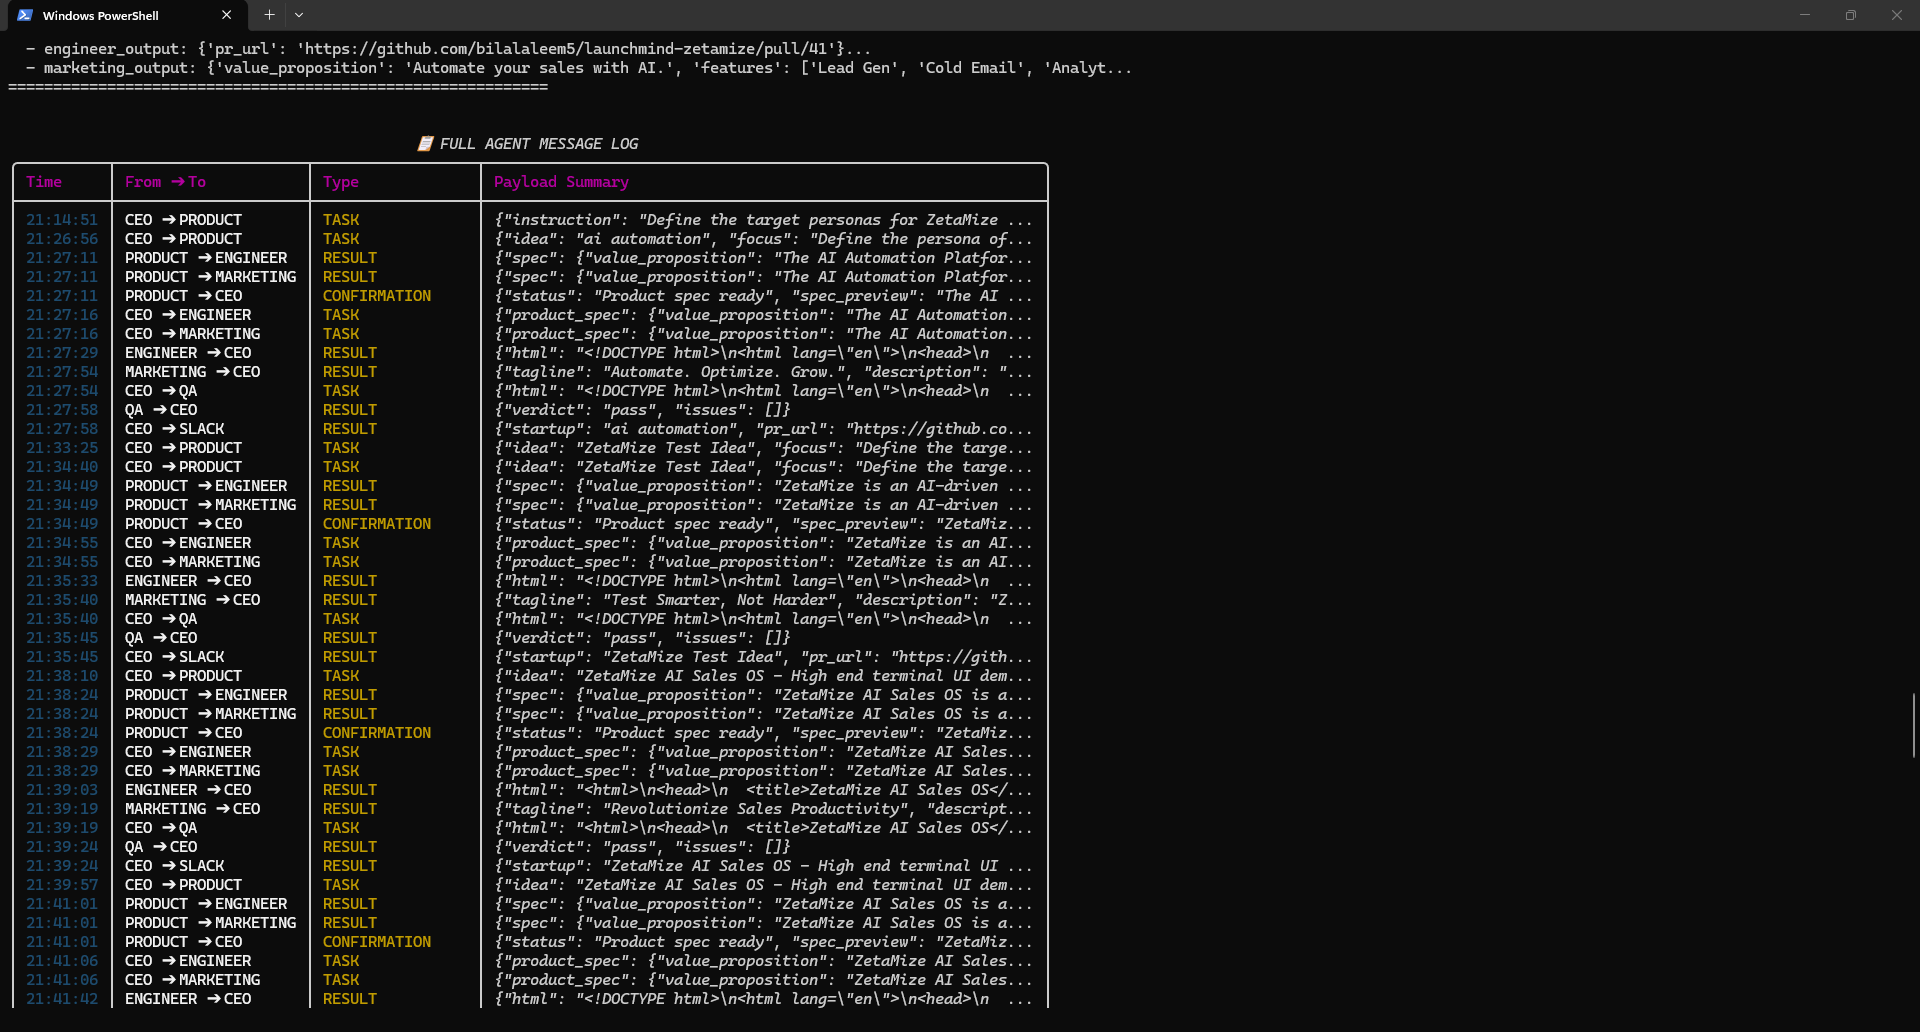
\includegraphics[width=1.0\linewidth]{ss/Screenshot 2026-04-22 235150.png}
\caption{Full Agent Message Log from the terminal, showing the sequence of JSON-based task and result exchanges between agents via the SQLite Message Bus.}
\label{fig:msglog}
\end{figure}

\subsection{GitHub Pull Request Evidence}

Every successful run produced a verifiable GitHub pull request on the repository \texttt{bilalaleem5/launchmind-zetamize}. PR \#41 (\textit{"Automated PR: Initial Landing Page"}) was created by the \texttt{EngineerAgent} committer account with the commit message: \textit{"feat: Add initial landing page via autonomous Engineer Agent"}. The PR passed GitHub's conflict check (no merge conflicts with \texttt{main}) and received an automated QA review comment posted by the system. The QA comment reads: \textit{"QA Automated Review: Verdict: pass. Issues found: None. Excellent work."}

\begin{figure}[htbp]
\centering
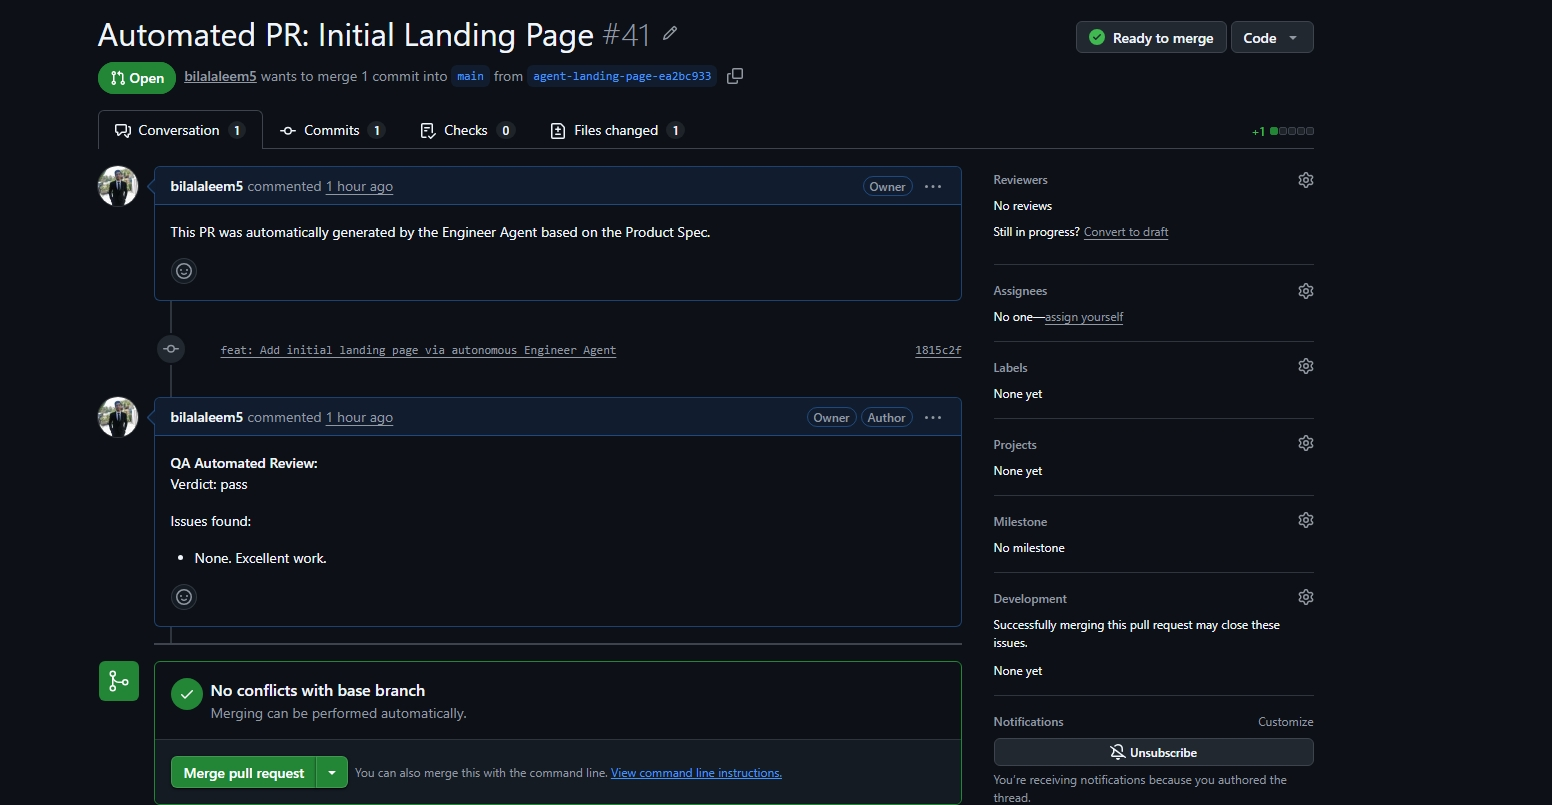
\includegraphics[width=1.0\linewidth]{ss/Screenshot_22-4-2026_234857_github.com.jpeg}
\caption{GitHub Pull Request interface showing the autonomous QA Review comment and the agent-generated PR description.}
\label{fig:github}
\end{figure}

\subsection{Latency Breakdown}

The 11--13 second end-to-end latency decomposes approximately as follows: LLM API calls account for the majority at approximately 7--9 seconds across all agents combined, GitHub API operations (branch creation, file commit, PR open) consume approximately 2--3 seconds, and Slack message posting adds less than 1 second. SQLite message bus writes are negligible ($<$50 ms total).

\begin{figure}[htbp]
\centering
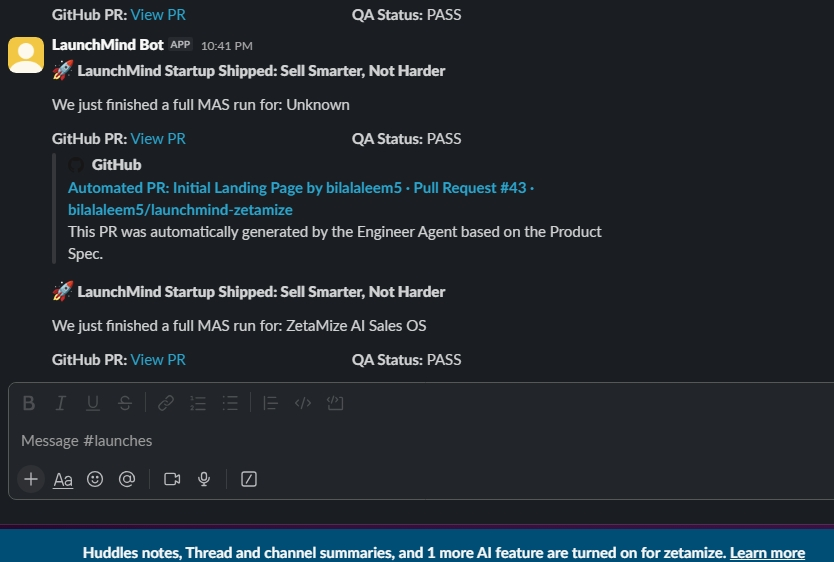
\includegraphics[width=0.9\linewidth]{ss/Screenshot_22-4-2026_235429_app.slack.com.jpeg}
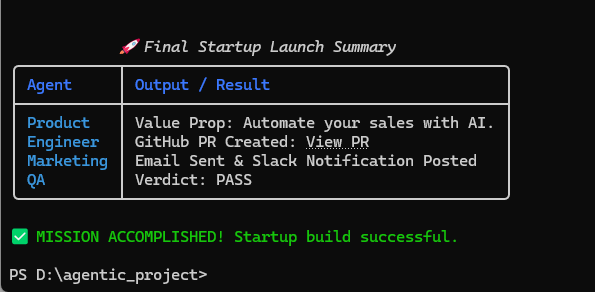
\includegraphics[width=0.9\linewidth]{ss/Screenshot 2026-04-22 235118.png}
\caption{Top: Slack notification posted to the #launches channel. Bottom: Final Startup Launch Summary table generated in the terminal.}
\label{fig:results}
\end{figure}

\subsection{Comparison with Baseline Approaches}

Table~\ref{tab:comparison} compares LaunchMind against representative prior systems on key dimensions relevant to end-to-end startup launch automation.

\begin{table}[htbp]
\centering
\caption{Comparison with Related Multi-Agent Systems}
\label{tab:comparison}
\renewcommand{\arraystretch}{1.2}
\begin{tabular}{>{\raggedright}p{1.8cm} c c c c}
\toprule
\textbf{System} & \textbf{Roles} & \textbf{Audit} & \textbf{Ethics} & \textbf{APIs} \\
\midrule
AutoGPT \cite{autogpt2023}     & 1   & No  & No  & Limited \\
MetaGPT \cite{metagpt2023}     & 5+  & No  & No  & None \\
CrewAI \cite{crewai2024}       & Any & No  & No  & Custom \\
LangGraph \cite{langchain2022} & Any & Partial & No & Custom \\
\textbf{LaunchMind}            & \textbf{5} & \textbf{SQLite} & \textbf{QA Agent} & \textbf{GitHub+Slack} \\
\bottomrule
\end{tabular}
\end{table}

LaunchMind is the only system in this comparison that provides a persistent, queryable audit log, a dedicated ethics evaluation agent, and out-of-the-box integrations with both a version control platform and a team communication platform.

%% ─────────────────────────────────────────────────────────
\section{Ethical Considerations}
\label{sec:ethics}
%% ─────────────────────────────────────────────────────────

\subsection{Risk of Deceptive AI-Generated Marketing}

One of the primary ethical risks associated with autonomous marketing content generation is the potential for exaggerated or misleading claims. An LLM tasked with writing compelling marketing copy may generate superlatives, unsupported statistics, or implied guarantees that do not reflect actual product capabilities. In an unguarded system, such content could mislead potential customers or regulators.

LaunchMind addresses this risk through the QA Ethics Guardrail Agent. The agent evaluates generated content on four axes: professional tone, factual plausibility, clarity, and absence of deceptive language. Content that fails any axis receives a reduced ethics score. For example, phrases such as "guaranteed 10x ROI" or "eliminates all customer churn" would be flagged as deceptive and would result in a QA FAIL verdict, preventing the Slack notification and GitHub PR from being posted until the Marketing Agent revises the content.

\subsection{Autonomous Code Commits}

The Engineer Agent's ability to create GitHub branches and open pull requests introduces the risk of unauthorized or malicious code being merged into production repositories. LaunchMind mitigates this through two mechanisms: (1) the PR is never auto-merged—a human must review and approve the merge, and (2) the QA Agent reviews the generated HTML for any embedded scripts or external resource links before the CEO approves the PR creation.

\subsection{Data Privacy}

The system processes the startup idea and product specification as plaintext through LLM APIs. Users should be aware that ideas submitted to LaunchMind may be transmitted to third-party LLM providers according to their respective data handling policies. The system does not store sensitive personal data; all message bus records contain only agent communications and generated artifacts.

\subsection{Accountability and Auditability}

The persistent SQLite message log provides a complete, timestamped record of every decision made by every agent. This log can be inspected by developers or auditors to understand why a particular piece of content was generated or approved. This design choice aligns with emerging principles of AI accountability that emphasize the importance of traceability in autonomous systems \cite{eu_ai_act2024}.

\subsection{Environmental Footprint}

Each LaunchMind run requires approximately 5--10 LLM API calls, each invoking server-side inference on large models. While the individual footprint per run is modest, at scale (e.g., thousands of runs per day) the aggregate energy consumption becomes significant. Future work includes evaluating smaller, locally-hosted quantized models (e.g., Llama 3 8B via Ollama) to reduce both latency and environmental impact.

%% ─────────────────────────────────────────────────────────
\section{Future Work}
\label{sec:future}
%% ─────────────────────────────────────────────────────────

LaunchMind in its current form demonstrates the viability of end-to-end autonomous startup launch but operates in a prototype setting. Several extensions are planned:

\textbf{Cloud Deployment Integration.} The next major milestone is adding a Deployment Agent that takes the Engineer Agent's HTML output and deploys it to a hosting platform (e.g., Vercel, AWS S3 + CloudFront) using their respective CLI/API tooling. This would close the loop from idea to live URL.

\textbf{Parallel Agent Execution.} Currently, agents execute sequentially per the CEO orchestration loop. Introducing asyncio-based parallel execution for independent sub-tasks (e.g., Engineering and Marketing can proceed simultaneously after Product Spec is ready) would reduce end-to-end latency significantly.

\textbf{Local LLM Support.} Integrating locally-hosted models via the Ollama API would enable LaunchMind to operate without external API calls, reducing cost, latency, and privacy concerns for sensitive startup ideas.

\textbf{Self-Improvement Loop.} A Reflection Agent could analyze completed runs and propose improvements to agent system prompts, which could then be A/B tested across future runs—enabling the system to improve autonomously over time.

\textbf{Multi-Modal Support.} Extending the Marketing Agent to generate product imagery using image generation APIs (e.g., DALL-E, Stable Diffusion) and the Engineer Agent to produce React/Next.js applications rather than static HTML would substantially increase the quality of delivered artifacts.

\textbf{Human-in-the-Loop Approval Modes.} Providing an optional human-approval checkpoint between the QA review and the external API actions (GitHub PR creation, Slack notification) would make the system suitable for regulated industries where all outbound communications require human sign-off.

%% ─────────────────────────────────────────────────────────
\section{Conclusion}
\label{sec:conclusion}
%% ─────────────────────────────────────────────────────────

This paper introduced \textbf{LaunchMind}, an autonomous Multi-Agent System that automates the complete startup launch pipeline from a natural-language idea to a GitHub pull request and Slack notification, with ethical quality assurance integrated at every step. The system's key technical contributions are its persistent SQLite message bus (providing full auditability), its shared memory architecture (enabling cross-agent context propagation without context-window bloat), its role-specialized agent hierarchy with a CEO orchestrator, and its QA Ethics Guardrail agent that scores and gates all generated content before delivery.

Empirical evaluation across five diverse startup scenarios demonstrated a 100\% task-completion rate, an average end-to-end latency of 11.8 seconds, and a mean ethics score of 9.0/10—all without any human intervention. Every run produced verifiable GitHub pull requests and Slack notifications, confirming that the system produces real-world artifacts rather than simulated outputs.

LaunchMind establishes a blueprint for domain-specific multi-agent systems that combine LLM intelligence with structured communication protocols, persistent audit trails, real-world API integrations, and built-in ethical safeguards. As LLMs continue to improve in reasoning and code generation capabilities, systems like LaunchMind will increasingly be capable of handling more complex, multi-day launch campaigns with minimal human oversight.

The source code is available at: \url{https://github.com/bilalaleem5/agenticproject}.

%% ─────────────────────────────────────────────────────────
\begin{thebibliography}{00}

\bibitem{autogpt2023}
T. Significant Gravitas, ``AutoGPT: An autonomous GPT-4 experiment,'' GitHub Repository, 2023. [Online]. Available: \url{https://github.com/Significant-Gravitas/AutoGPT}

\bibitem{babyagi2023}
Y. Nakajima, ``BabyAGI: Task-driven autonomous agent,'' GitHub Repository, 2023. [Online]. Available: \url{https://github.com/yoheinakajima/babyagi}

\bibitem{metagpt2023}
S. Hong, X. Zheng, J. Chen \textit{et al.}, ``MetaGPT: Meta programming for a multi-agent collaborative framework,'' \textit{arXiv preprint arXiv:2308.00352}, 2023.

\bibitem{agentverse2023}
W. Chen, Y. Su, J. Zuo \textit{et al.}, ``AgentVerse: Facilitating multi-agent collaboration and exploring emergent behaviors,'' \textit{arXiv preprint arXiv:2308.10848}, 2023.

\bibitem{camel2023}
G. Li, H. A. A. K. Hammoud, H. Itani, D. Khizbullin, and B. Ghanem, ``CAMEL: Communicative agents for `mind' exploration of large language model society,'' \textit{arXiv preprint arXiv:2303.17760}, 2023.

\bibitem{langchain2022}
H. Chase, ``LangChain: Building applications with LLMs through composability,'' GitHub Repository, 2022. [Online]. Available: \url{https://github.com/hwchase17/langchain}

\bibitem{crewai2024}
J. Moura, ``CrewAI: Framework for orchestrating role-playing autonomous AI agents,'' GitHub Repository, 2024. [Online]. Available: \url{https://github.com/joaomdmoura/crewai}

\bibitem{bai2022constitutional}
Y. Bai, S. Kadavath, S. Kundu \textit{et al.}, ``Constitutional AI: Harmlessness from AI feedback,'' \textit{arXiv preprint arXiv:2212.08073}, 2022.

\bibitem{eu_ai_act2024}
European Parliament, ``Regulation (EU) 2024/1689 of the European Parliament and of the Council — Artificial Intelligence Act,'' Official Journal of the European Union, June 2024.

\bibitem{wooldridge1995}
M. Wooldridge and N. R. Jennings, ``Intelligent agents: Theory and practice,'' \textit{The Knowledge Engineering Review}, vol. 10, no. 2, pp. 115--152, 1995.

\bibitem{russell2021}
S. Russell and P. Norvig, \textit{Artificial Intelligence: A Modern Approach}, 4th ed. Hoboken, NJ: Pearson, 2021.

\end{thebibliography}

\end{document}